\chapter{Diseño del \emph{hardware}}

\section{Introducción}

\emph{The Embedded Development Kit} (EDK) es un entorno de desarrollo integrado
para el diseño de sistemas empotrados. Este kit preconfigurado incluye
\emph{Xilinx Platform Studio} y el kit de desarrollo de software, así como toda
la documentación e IP que requieren para el diseño de FPGAs con procesadores
PowerPC integrados.

\section{Plataforma de \emph{hardware}}

La plataforma de \emph{hardware}, incluye uno o más procesadores, además de
una variedad de periféricos y los bloques de memoria. Estos bloques utilizan una
red de interconexión para comunicarse. El comportamiento de cada procesador o
núcleo periférico se pueden personalizar\cite{Beto}.


Para el diseño del \emph{hardware} se hará uso de la herramienta \emph{Xilinx
EDK 8.2.02 Build EDK\_Im\_Sp2.4}, para la detalles de la instalación se puede
consultar el \emph{Apéndice A}.

\section{Diseño y configuración del sistema de \emph{hardware}}

\begin{enumerate}
 \item Creación de un nuevo Proyecto, \emph{figura} \ref{Nuevo proyecto en
Xilinx EDK}.
  \begin{figure}[h!] 
  \centering
  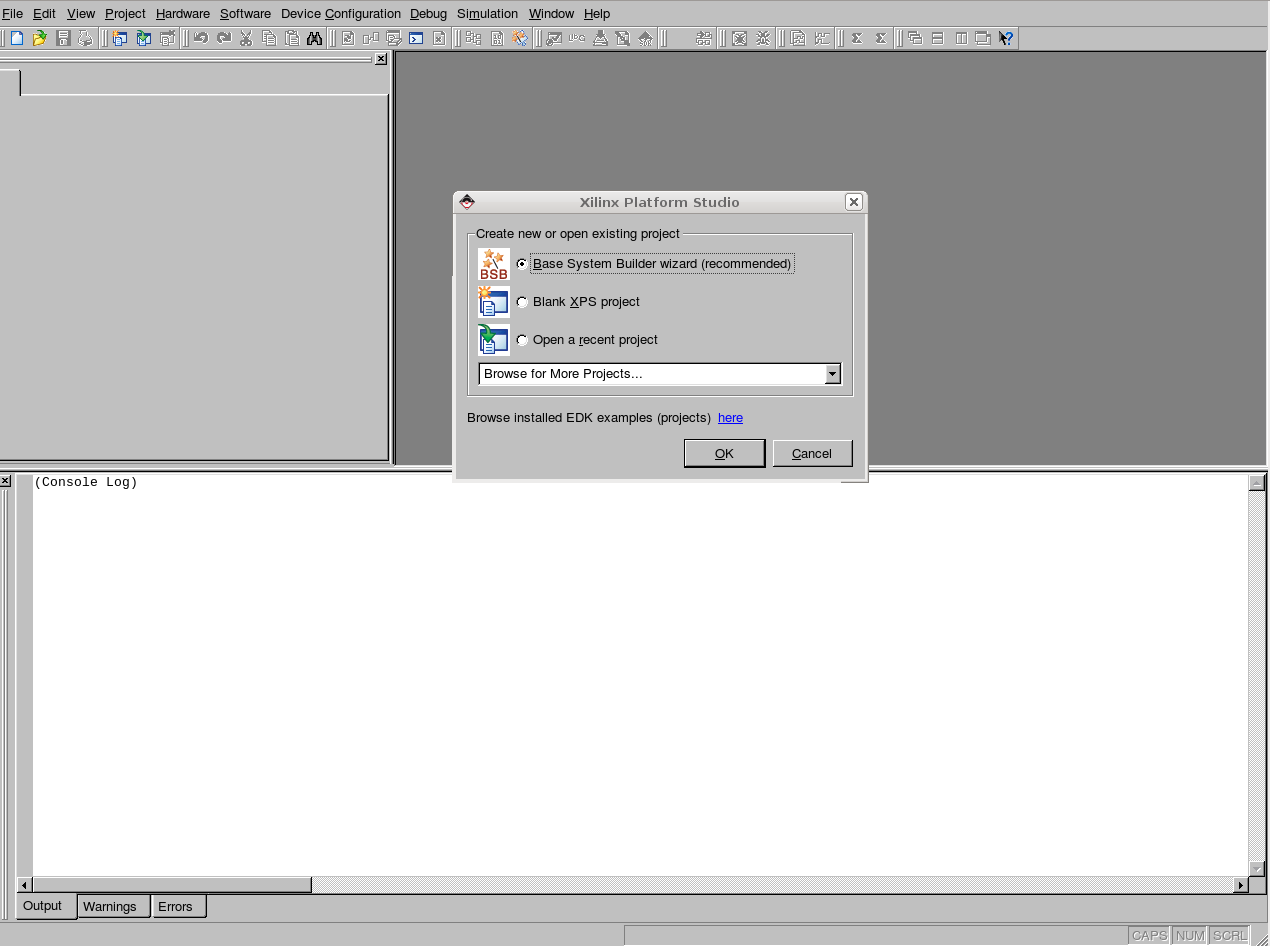
\includegraphics[scale=.25]{./figuras/EDK0.png}
  % capas.png: 607x522 pixel, 72dpi, 21.41x18.41 cm, bb=0 0 607 522
  \caption{Nuevo proyecto en Xilinx EDK}
  \label{Nuevo proyecto en Xilinx EDK}
  \end{figure}
 \item Selección del directorio destino, \emph{figura} \ref{Selección del
directorio destino}.
  \begin{figure}[h!] 
  \centering
  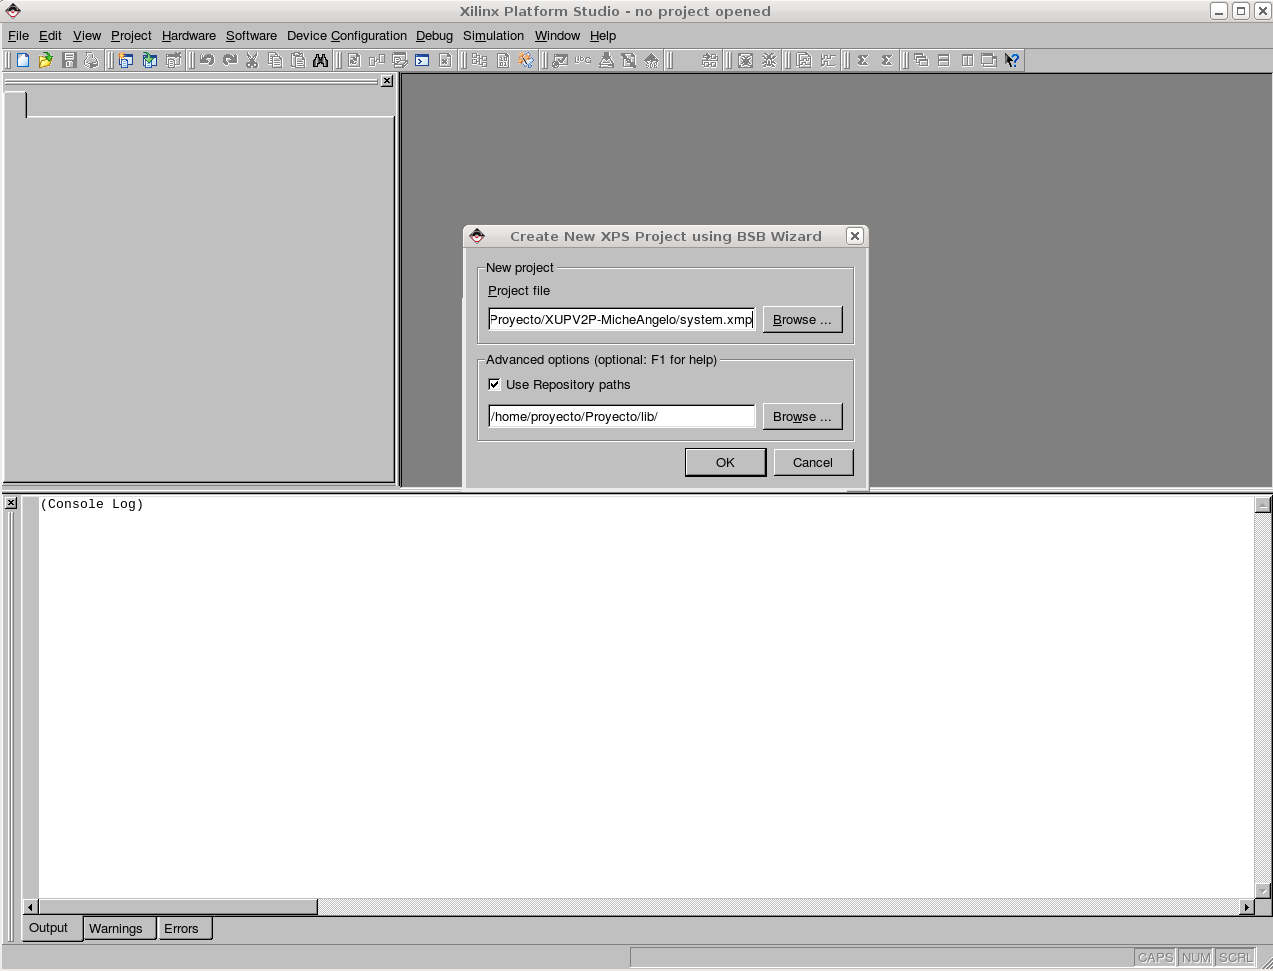
\includegraphics[scale=.25]{./figuras/EDK1.png}
  % capas.png: 607x522 pixel, 72dpi, 21.41x18.41 cm, bb=0 0 607 522
  \caption{Selección del directorio destino}
  \label{Selección del directorio destino}
  \end{figure}
 \item Ajuste del \emph{Project Peripheral Repositories} a los contenidos\\
``lib\_xupv2p\_edk\_10\_1\_sp3.zip'' que puede descargarse de la pagina de
 \emph{diligent}
 \url{http://www.digilentinc.com/Products/Detail.cfm?Prod=XUPV2P}. 
  Este archivo es necesario para que XPS reconozca las características de la
tarjeta, \emph{figura} \ref{Selección del directorio destino}.
 \item Seleccione crear un nuevo diseño con \emph{I would like to create a new
design} como se muestra en la \emph{figura} \ref{Selección de un nuevo diseño}.
  \begin{figure}[h!] 
  \centering
  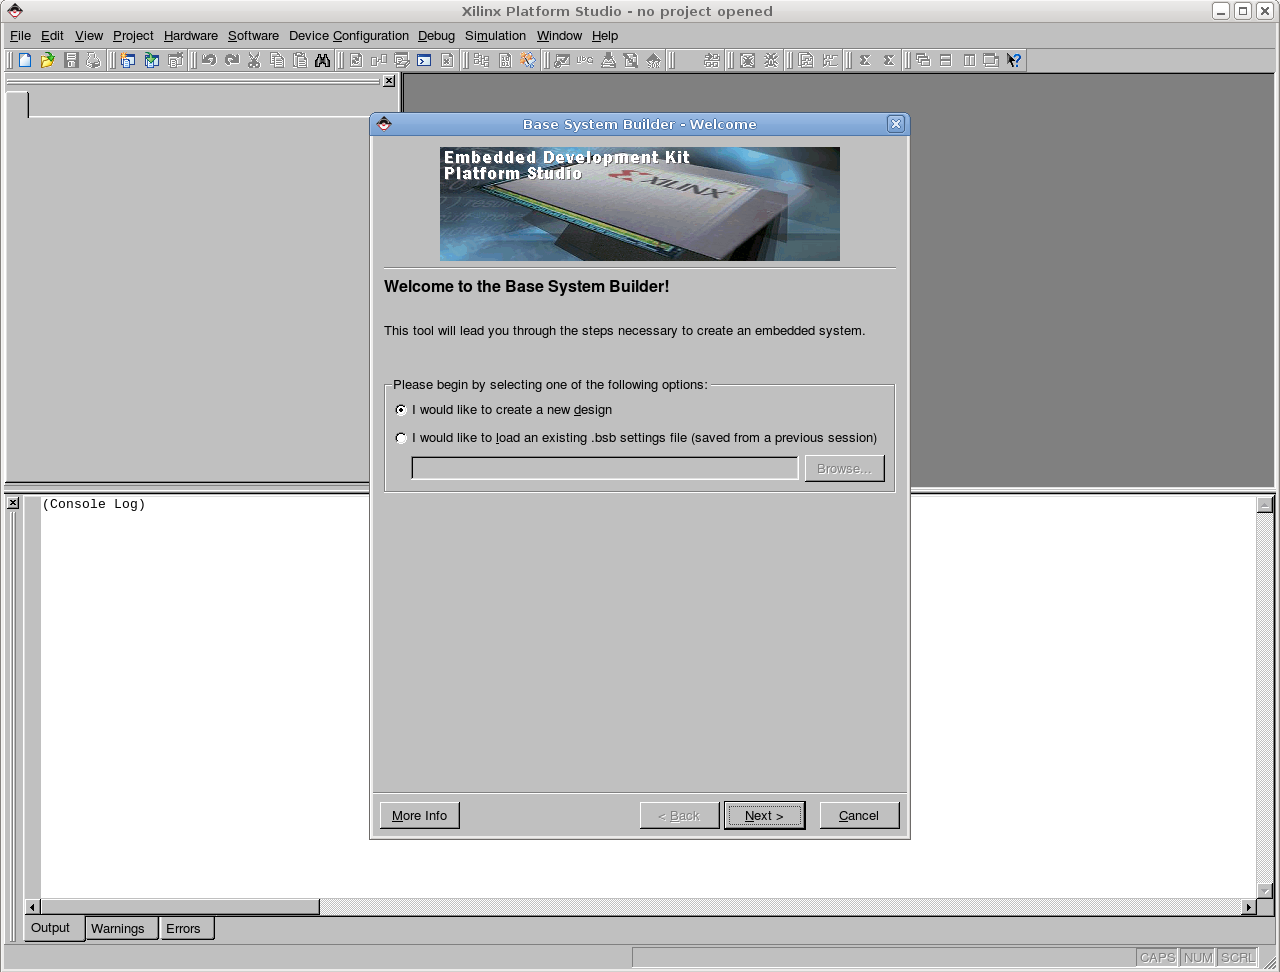
\includegraphics[scale=.25]{./figuras/EDK2.png}
  % capas.png: 607x522 pixel, 72dpi, 21.41x18.41 cm, bb=0 0 607 522
  \caption{Selección de un nuevo diseño}
  \label{Selección de un nuevo diseño}
  \end{figure}
 
  
 \item Seleccione Vendor ``Xilinx'' esto ajustará automáticamente el modelo
 adecuado: ``XUP Virtex-II Pro Development System'', \emph{figura}
\ref{Selección de tarjeta de desarrollo}.
  \begin{figure}[h!] 
  \centering
  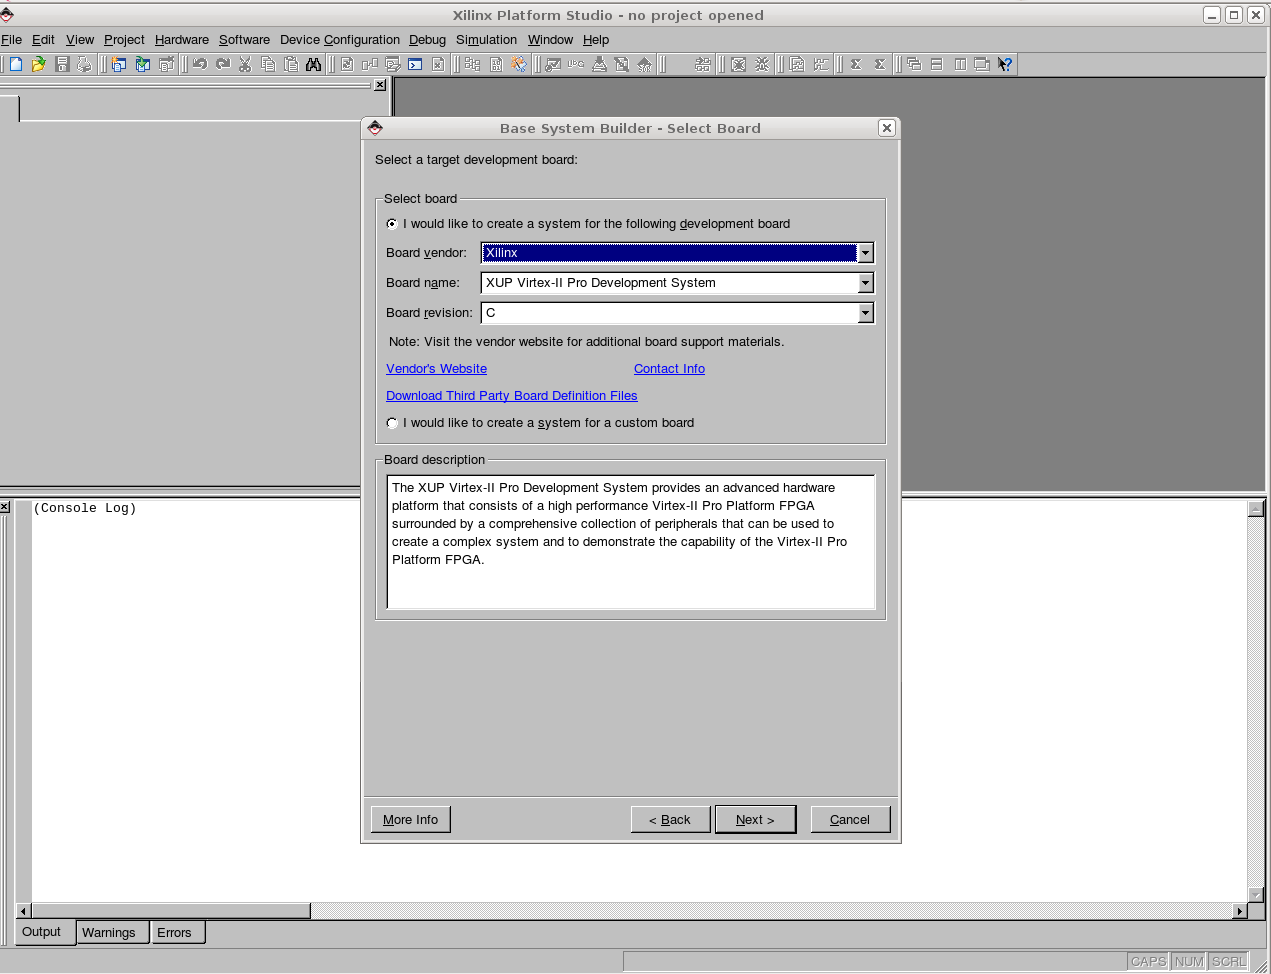
\includegraphics[scale=.25]{./figuras/EDK3.png}
  % capas.png: 607x522 pixel, 72dpi, 21.41x18.41 cm, bb=0 0 607 522
  \caption{Selección de tarjeta de desarrollo}
  \label{Selección de tarjeta de desarrollo}
  \end{figure}
    
  \item Seleccione PowerPC, como se menciona en las características de la
tarjeta de desarrollo la tarjeta XUPV2P cuenta con un procesador PowerPC405 sin
unidad de punto flotante, \emph{figura}
\ref{Selección de procesador}.
  \begin{figure}[h!] 
  \centering
  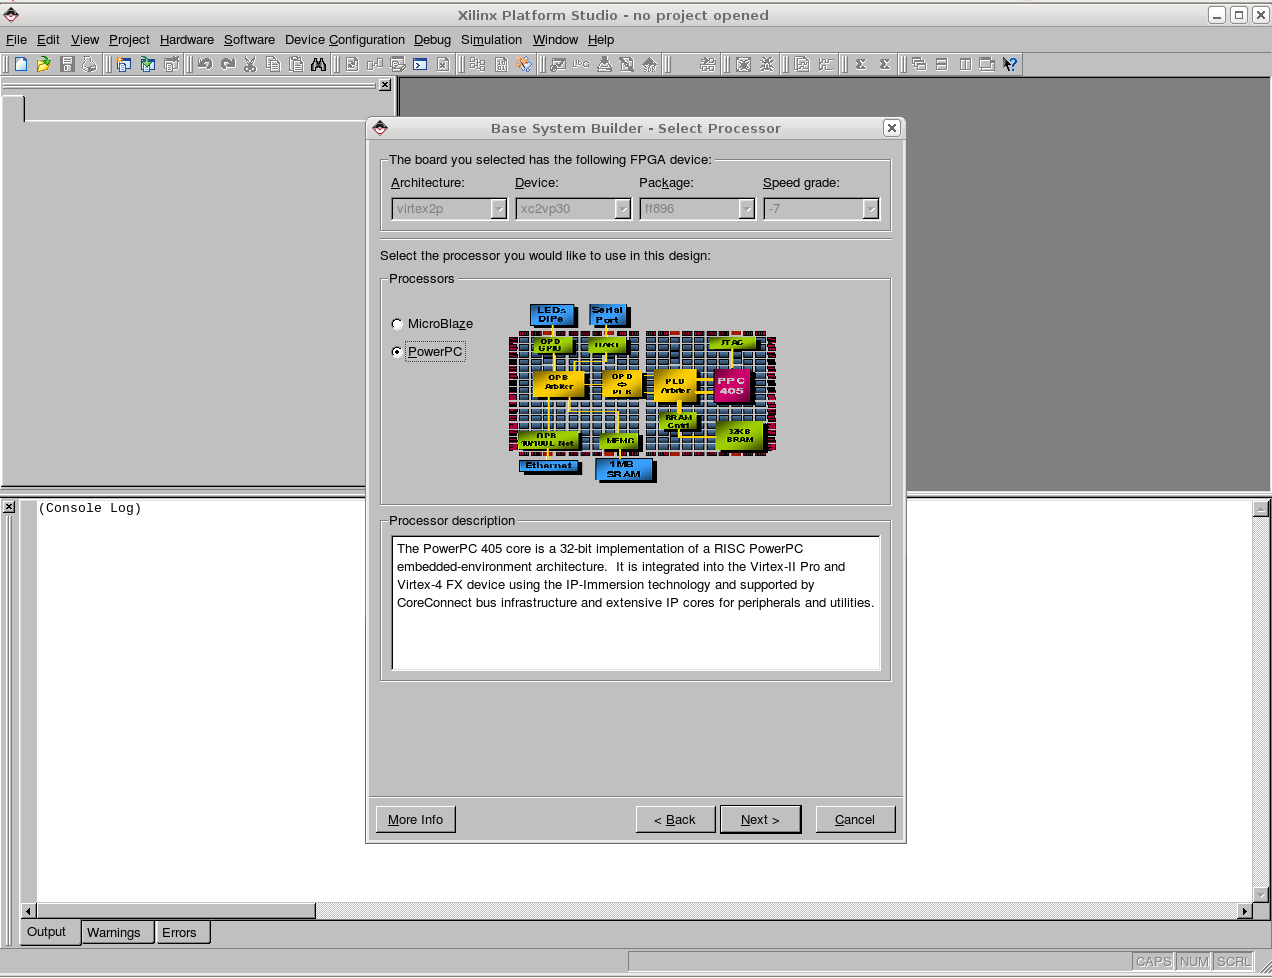
\includegraphics[scale=.25]{./figuras/EDK4.png}
  % capas.png: 607x522 pixel, 72dpi, 21.41x18.41 cm, bb=0 0 607 522
  \caption{Selección de procesador}
  \label{Selección de procesador}
  \end{figure}
 
  
 \item Aumentar la frecuencia de la CPU a 300 MHz. Habilitar la caché. Es
posible aumentar la frecuencia a 400MHz en pasos posteriores, pero requiere
consideraciones especiales y no es posible aumentar la velocidad del bus
principal (100MHz) así que el aumento de la frecuencia no incide
significativamente en el rendimiento, \emph{figura}
\ref{Configurando el procesador PowerPC}.
  \begin{figure}[h!] 
  \centering
  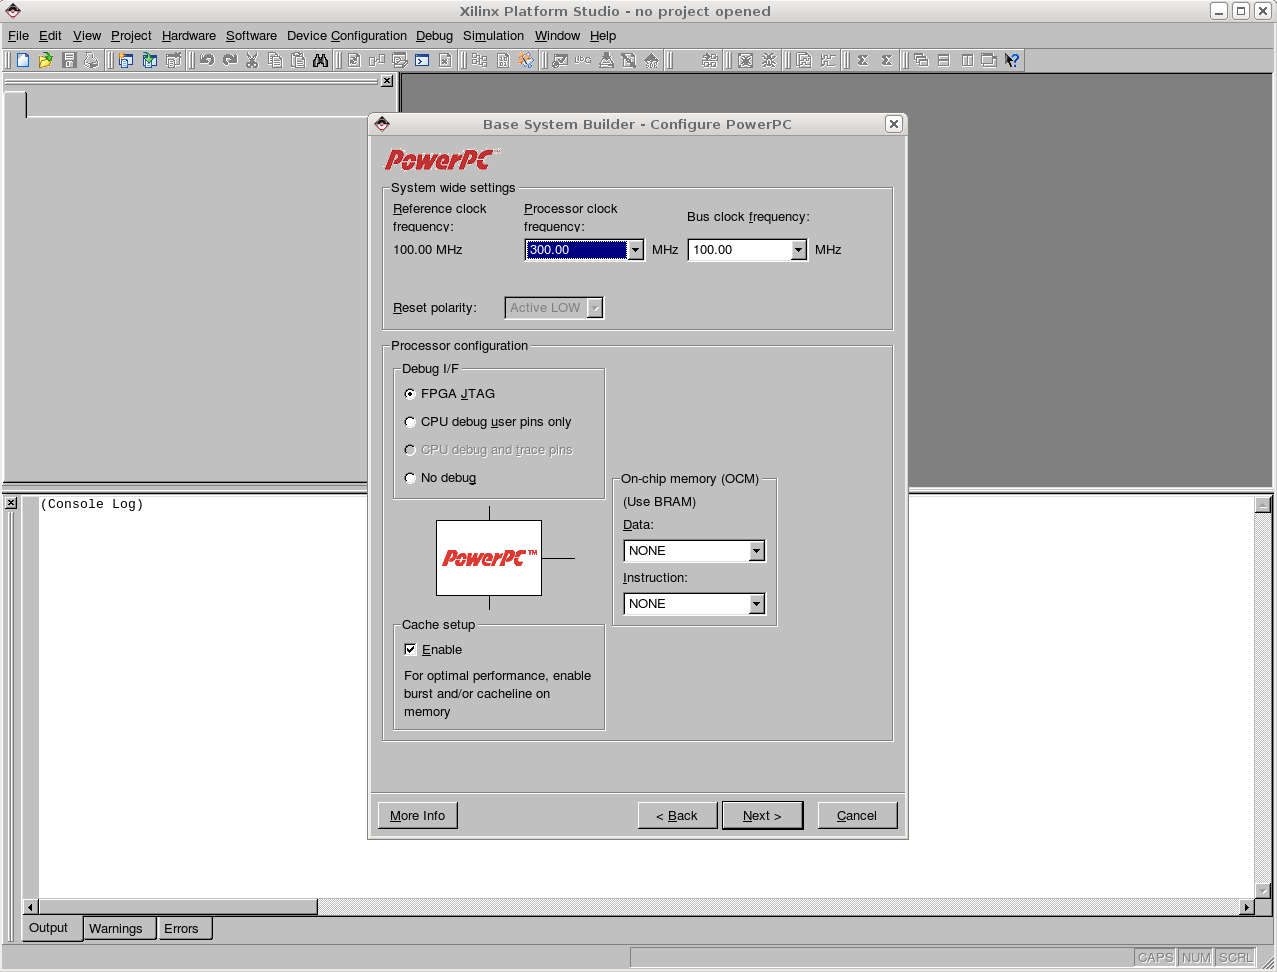
\includegraphics[scale=.25]{./figuras/EDK5.png}
  % capas.png: 607x522 pixel, 72dpi, 21.41x18.41 cm, bb=0 0 607 522
  \caption{Configurando el procesador PowerPC}
  \label{Configurando el procesador PowerPC}
  \end{figure}
  
  
\item Aumentar la velocidad de transmisión RS232 a 9600 Baudios y seleccione
\emph{Use interrupt} para cada periférico. Es posible aumentar la velocidad de
transmisión, esta es la minima recomendada, \emph{figura}
\ref{Configuracón del RS232}.
  \begin{figure}[h!] 
  \centering
  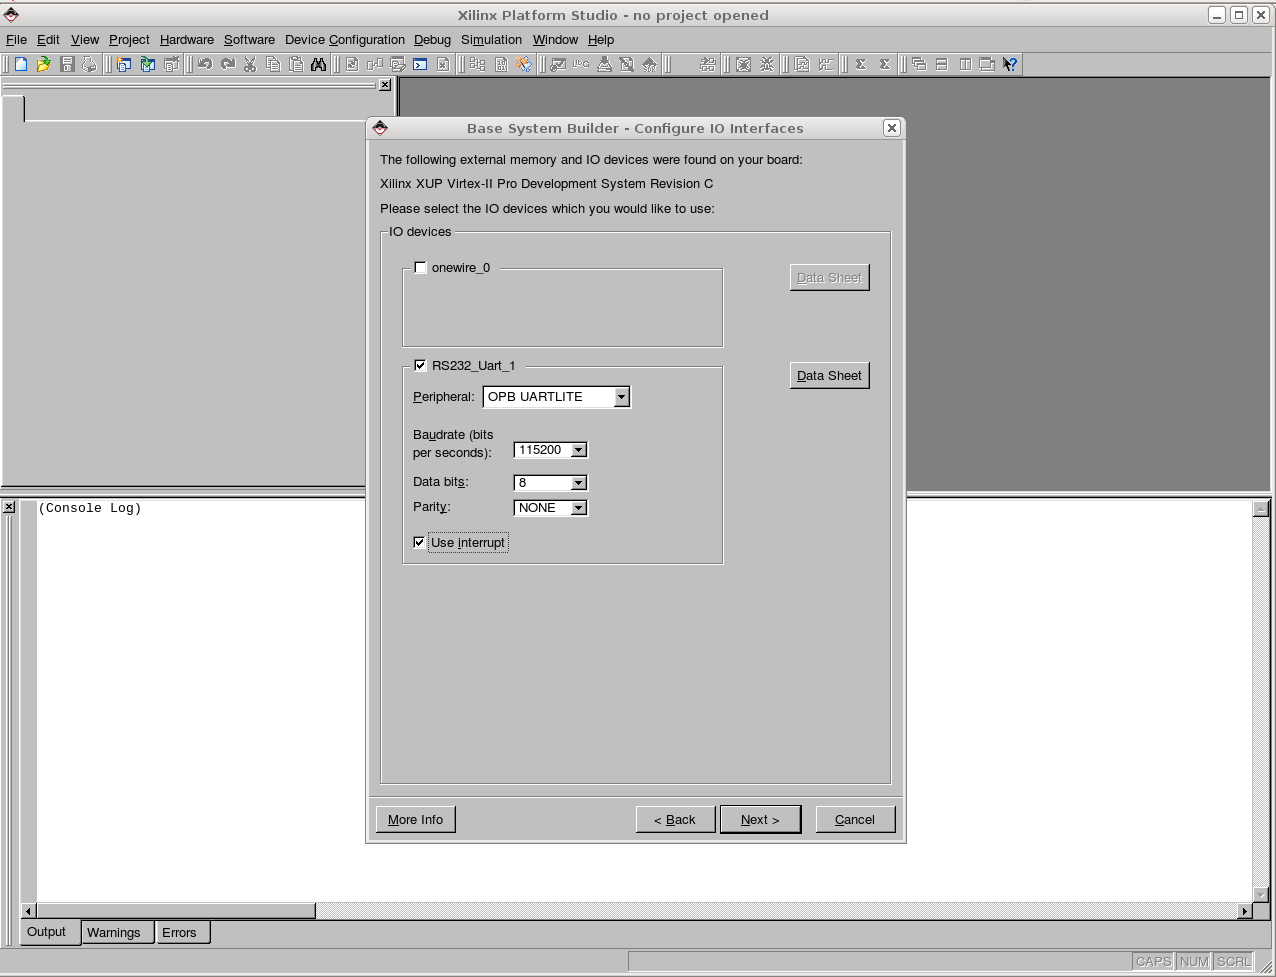
\includegraphics[scale=.25]{./figuras/EDK6.png}
  % capas.png: 607x522 pixel, 72dpi, 21.41x18.41 cm, bb=0 0 607 522
  \caption{Configuracón del RS232}
  \label{Configuracón del RS232}
  \end{figure}
 
   
\item Seleccione ``Ethernet\_MAC'' y seleccione ``OPB ETHERNETLITE'' y Active
interrupción. Este ``OPB ETHERNETLITE'' se puede obtener desde la pagina de la
empresa ``Xilinx'' sin costo alguno, en la  \emph{figura}
\ref{lic} se puede ver el estado de la licencia.
  \begin{figure}[h!] 
  \centering
  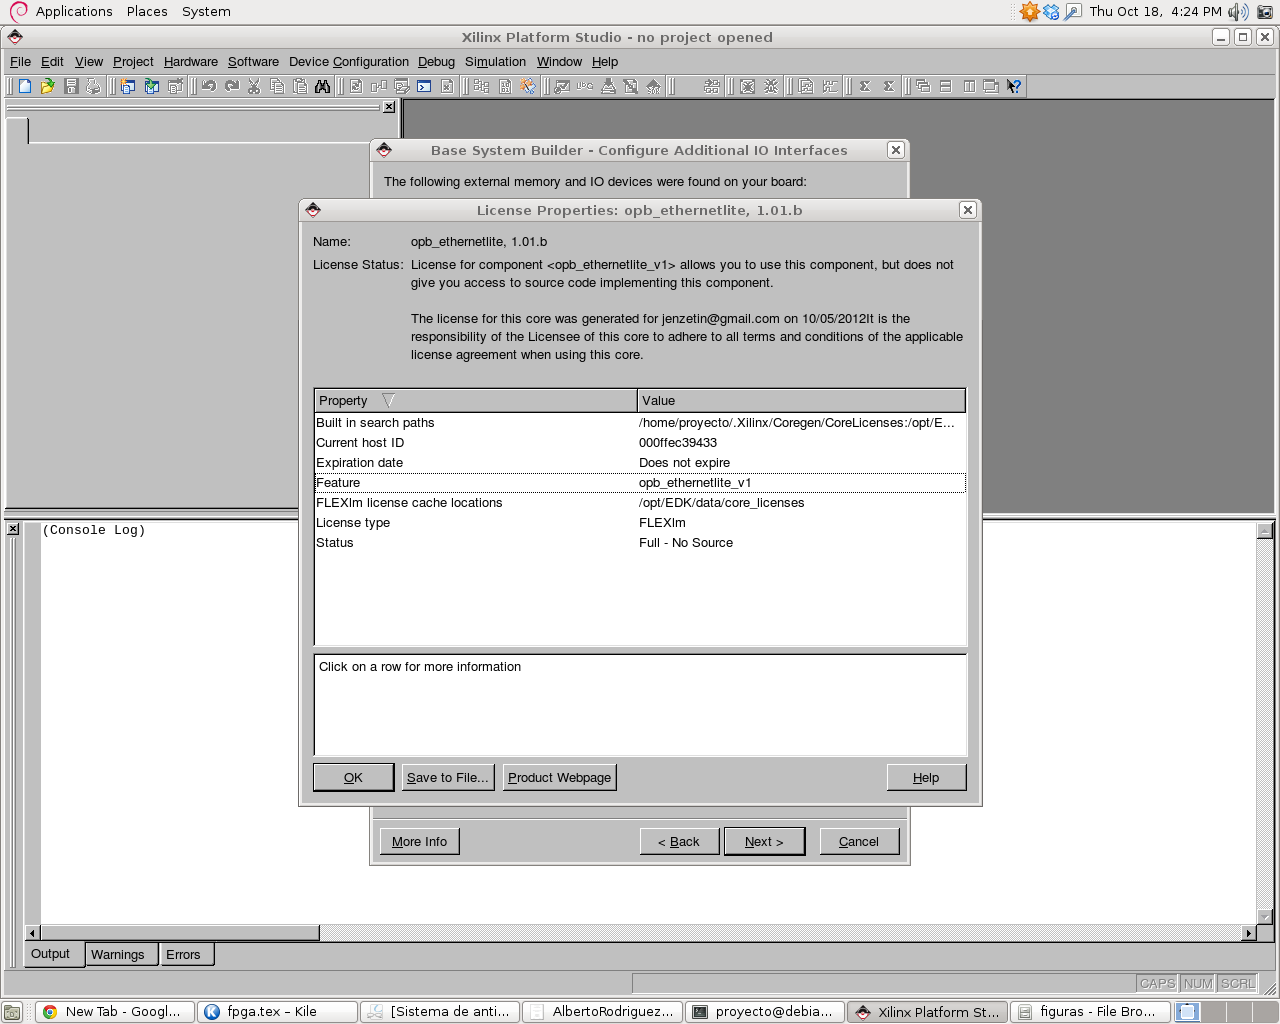
\includegraphics[scale=.25]{./figuras/lic.png}
  % capas.png: 607x522 pixel, 72dpi, 21.41x18.41 cm, bb=0 0 607 522
  \caption{Estado de la licencia}
  \label{lic}
  \end{figure}
  
  
\item Seleccione SysACE\_CompactFlash y active interrupción,  \emph{figura}
\ref{Selección del SysACE}.
  \begin{figure}[h!] 
  \centering
  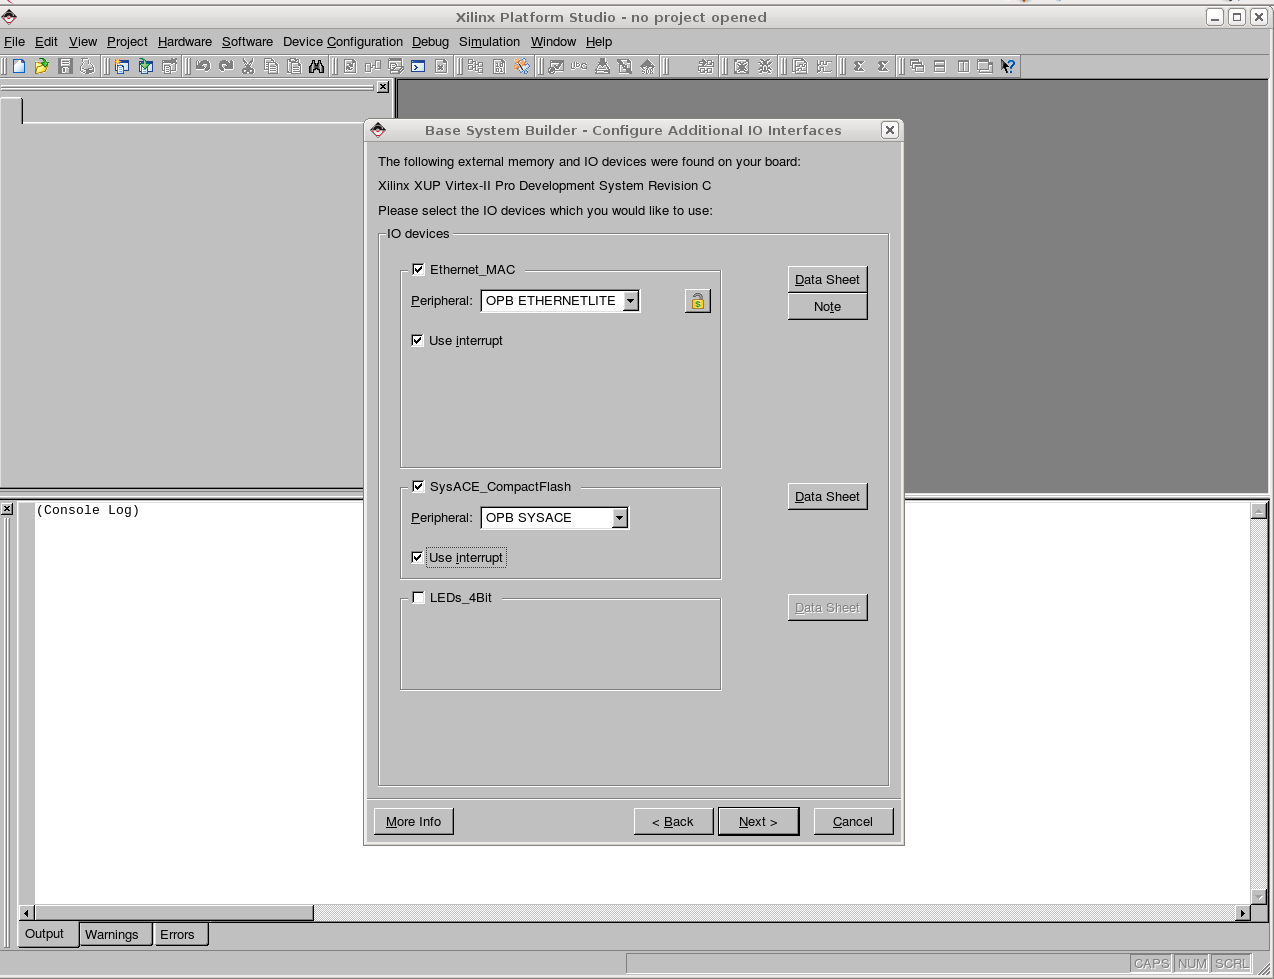
\includegraphics[scale=.25]{./figuras/EDK7.png}
  % capas.png: 607x522 pixel, 72dpi, 21.41x18.41 cm, bb=0 0 607 522
  \caption{Selección del  Ethernet\_MAC y SysACE}
  \label{Selección del SysACE}
  \end{figure}
  
  
\item Seleccione la memoria DDR disponible, en mi caso 256MB. Deseleccione el
resto del hardware. Deseleccione la interrupción,  \emph{figura}\ref{Selección
de Dispositivo de Memoria DDR}.
  \begin{figure}[h!] 
  \centering
  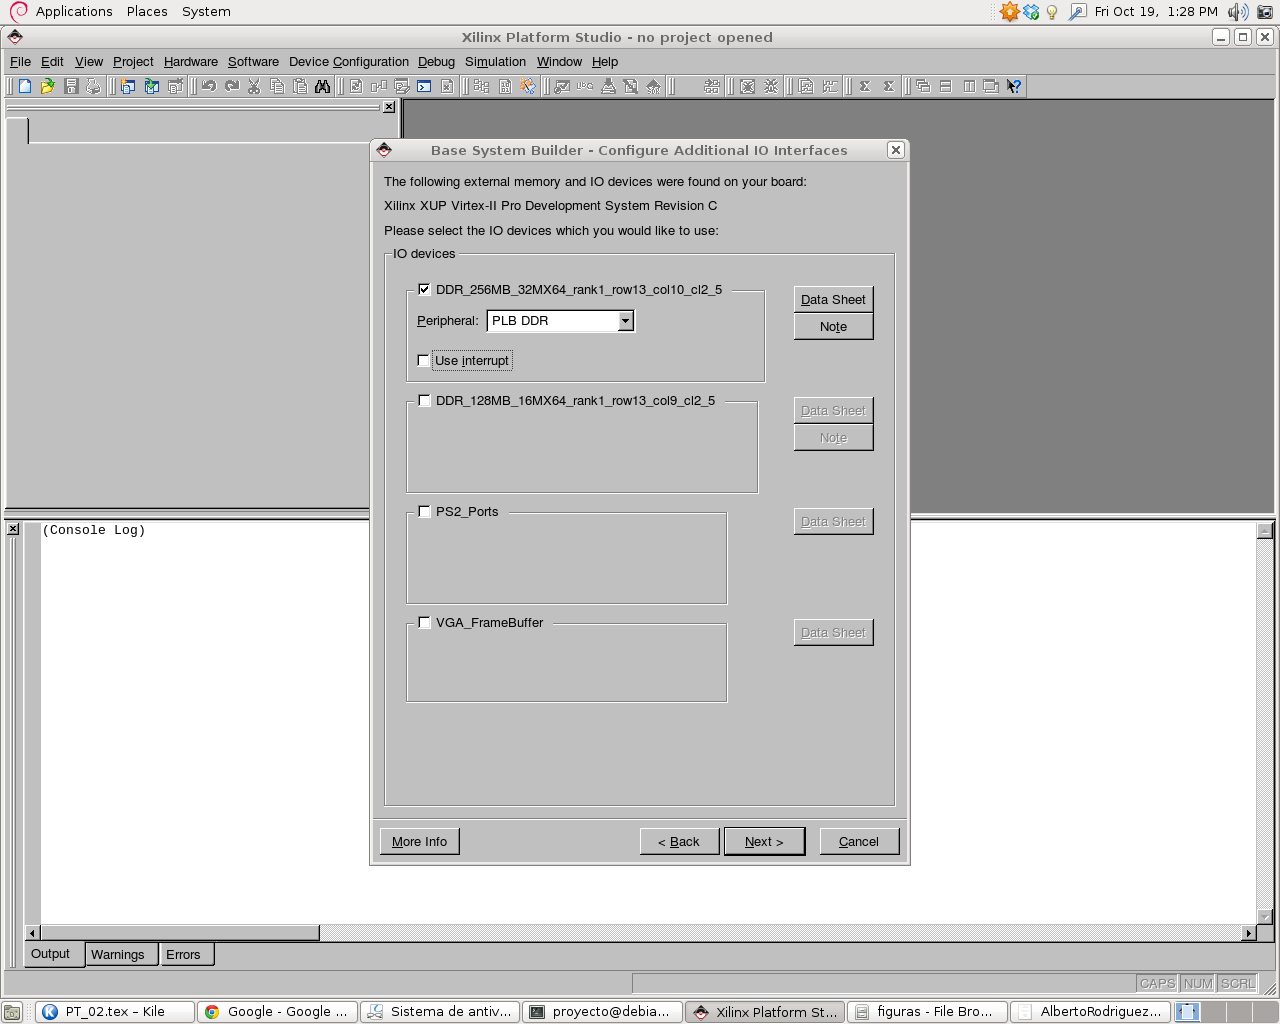
\includegraphics[scale=.25]{./figuras/EDK8.png}
  % capas.png: 607x522 pixel, 72dpi, 21.41x18.41 cm, bb=0 0 607 522
  \caption{Selección de Dispositivo de Memoria DDR}
  \label{Selección de Dispositivo de Memoria DDR}
  \end{figure}
  
  
\item Elija 128 kB de RAM. No elija 8 kB, ya que esto no es compatible con el
Virtex- II PRO. Se debe de contar  con BRAM para que el \emph{bootloop} del
procesador PPC405 funcione correctamente. El \emph{bootloop} es el proceso
mediante el cual procesador busca y carga el programa que ejecutara desde la
dirección \emph{0xfffffffc}, esto se muestra en la
\emph{figura}\ref{Configuracón de BRAM}.
  \begin{figure}[h!] 
  \centering
  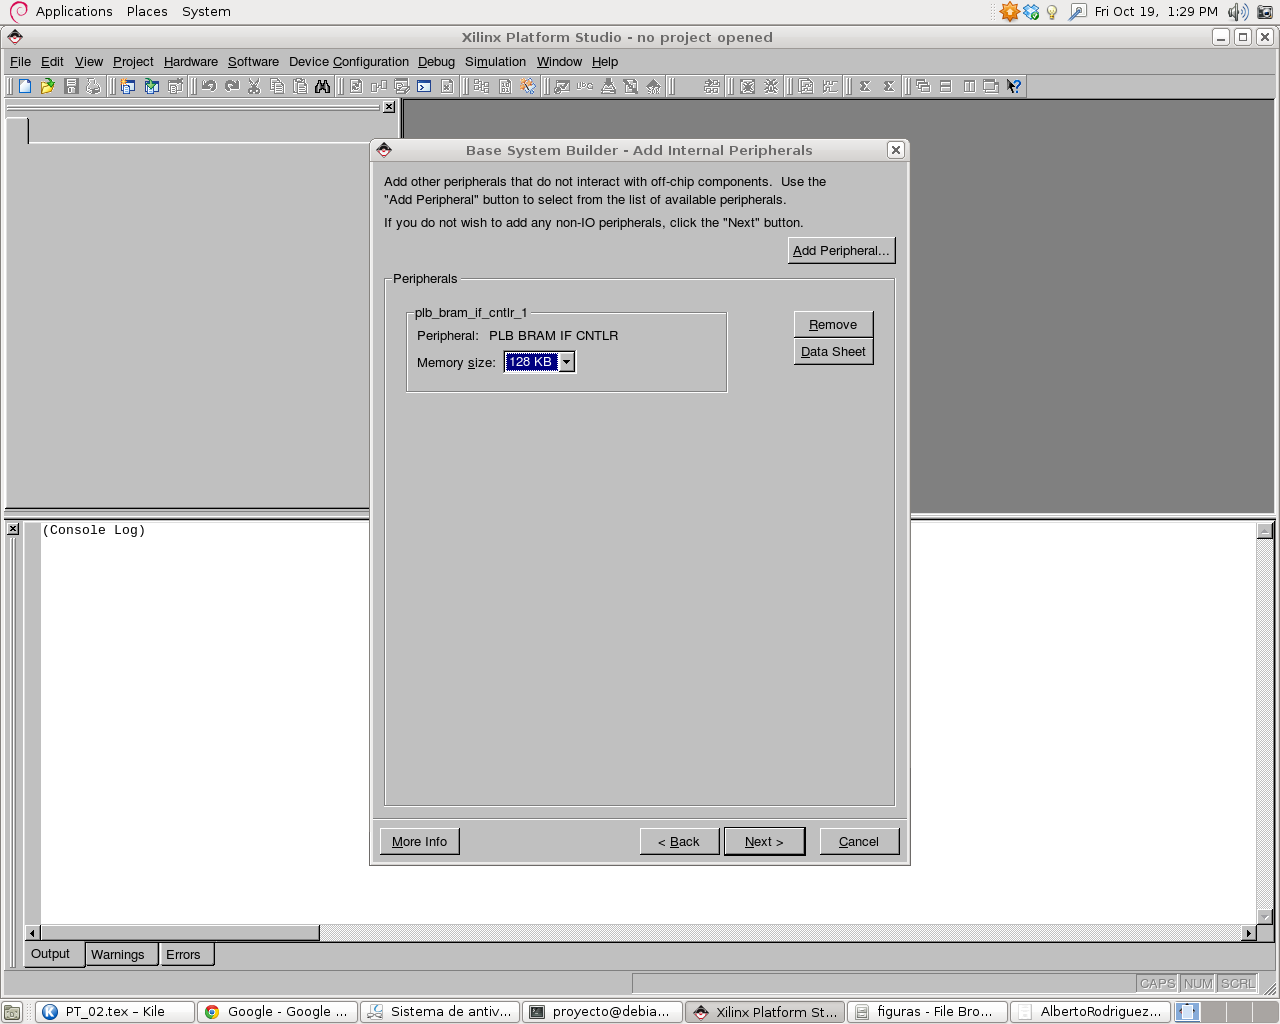
\includegraphics[scale=.25]{./figuras/EDK9.png}
  % capas.png: 607x522 pixel, 72dpi, 21.41x18.41 cm, bb=0 0 607 522
  \caption{Selección de Dispositivo de Memoria DDR}
  \label{Configuracón de BRAM}
  \end{figure}

\item Habilitar ICACHE y DCACHE (Instrucciones y datos respectivamente) para
DDR\_SRAM. En código C de Xilinx esto permite usar las macros
``XCache\_EnableICache'' y ''XCache\_EnableDCache'' para habilitar la cache y
teóricamente aumentar el desempeño, la configuración se mustra en la
\emph{figura}\ref{Selección de lineas de Caché}.
  \begin{figure}[h!] 
  \centering
  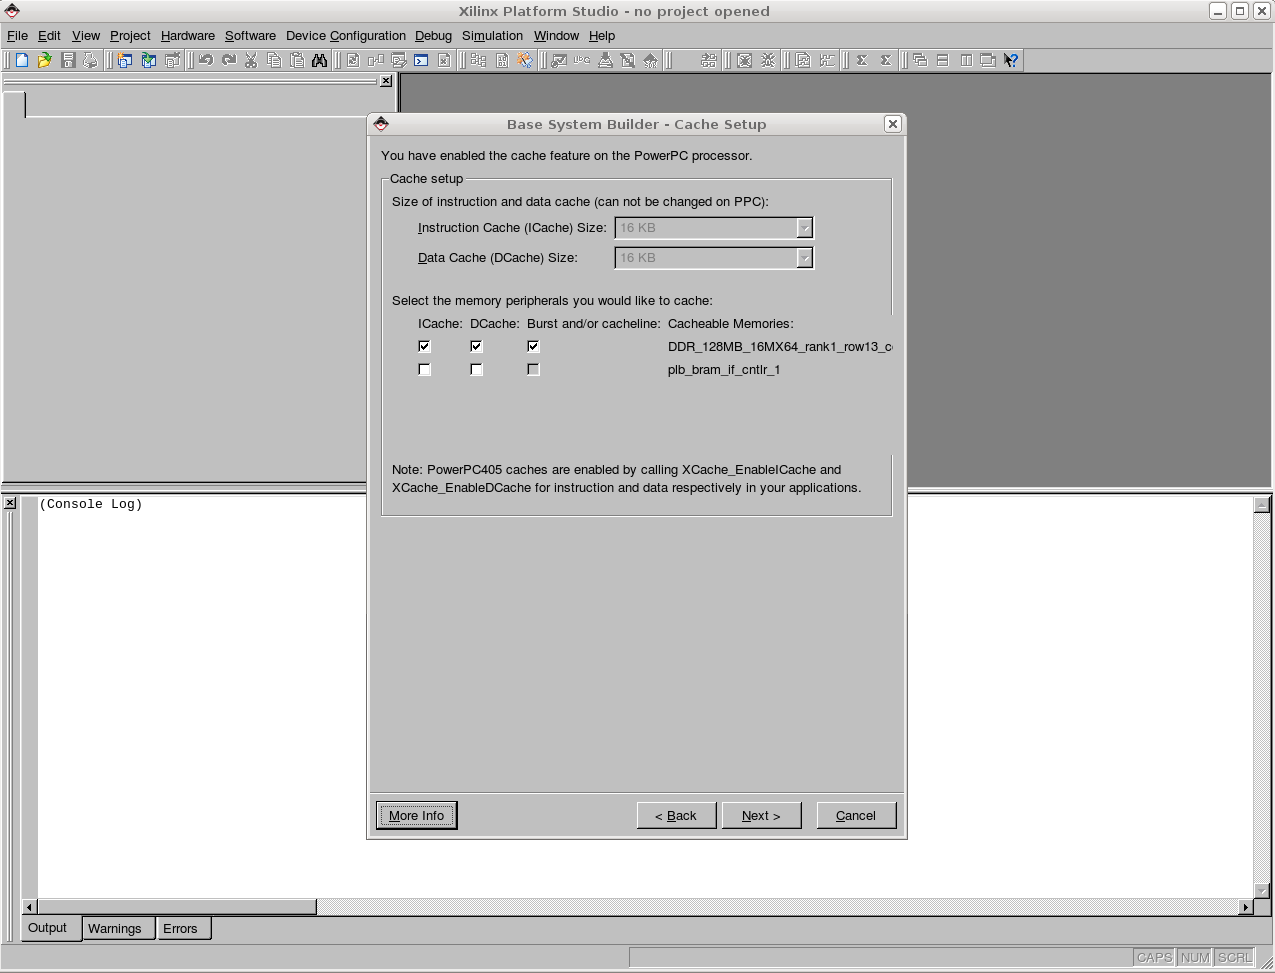
\includegraphics[scale=.25]{./figuras/EDK10.png}
  % capas.png: 607x522 pixel, 72dpi, 21.41x18.41 cm, bb=0 0 607 522
  \caption{Selección de lineas de Caché}
  \label{Selección de lineas de Caché}
  \end{figure}
  
  
\item Seleccione \emph{TestMemory}, \emph{TestMemory} permitirá saber que la
plataforma hardware funciona aunque sea en un nivel muy básico. Ya no es
necesario configurar más \emph{hardware}, esto se muestra en la
\emph{figura}\ref{Selección de programa de prueba}.
  \begin{figure}[h!] 
  \centering
  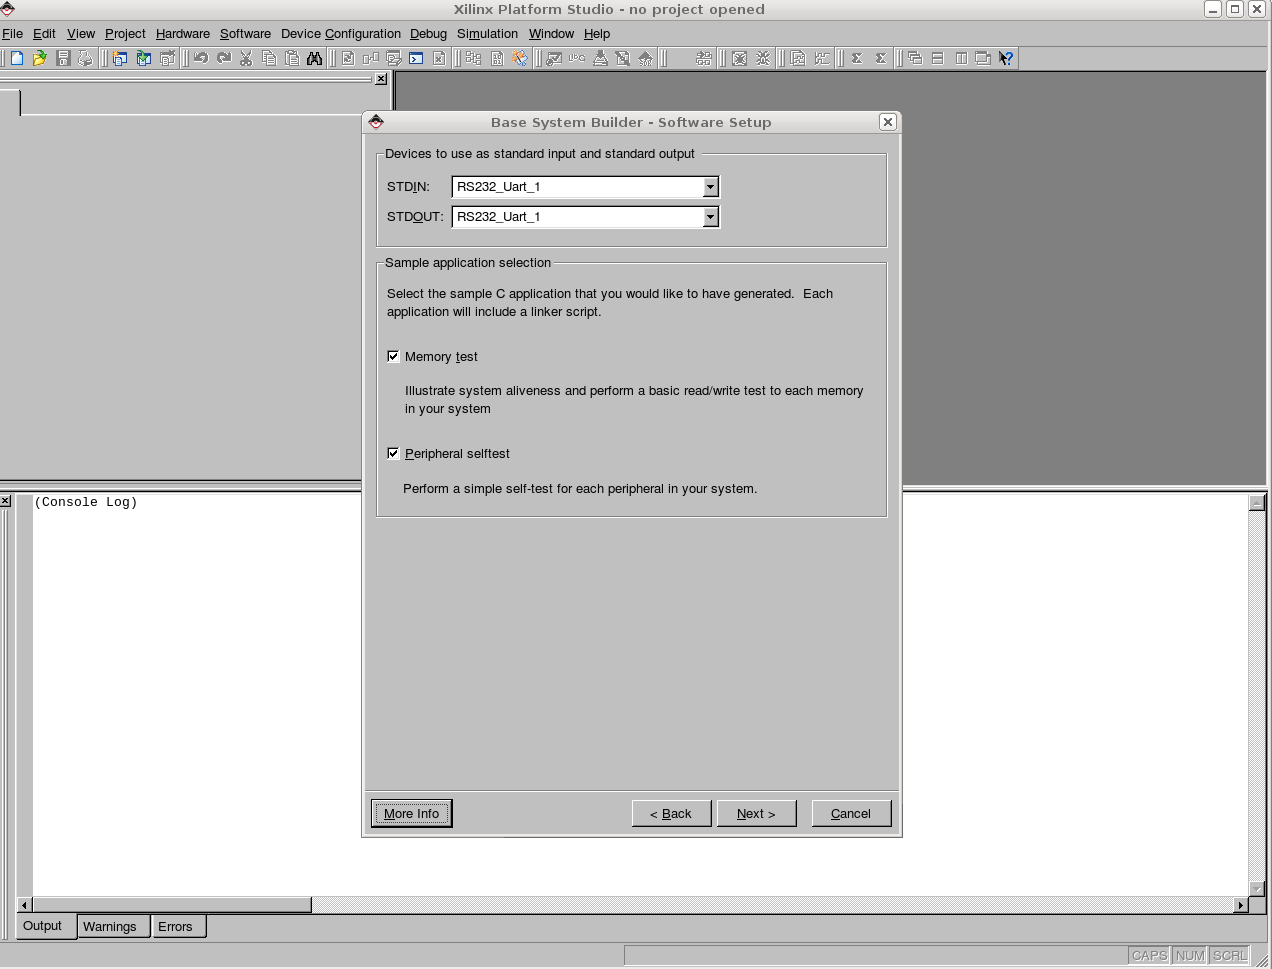
\includegraphics[scale=.25]{./figuras/EDK11.png}
  % capas.png: 607x522 pixel, 72dpi, 21.41x18.41 cm, bb=0 0 607 522
  \caption{Selección de programa de prueba}
  \label{Selección de programa de prueba}
  \end{figure}
  
  
\item Mantenga los datos, instrucciones y \emph{Heap/Stack} en la BRAM. Es
necesario para poder ser alcanzados en el \emph{BootLoop} del PPC405,
\emph{hardware}, esto se muestra en la
\emph{figura}\ref{Selección de división del programa en memoria}.
  \begin{figure}[h!] 
  \centering
  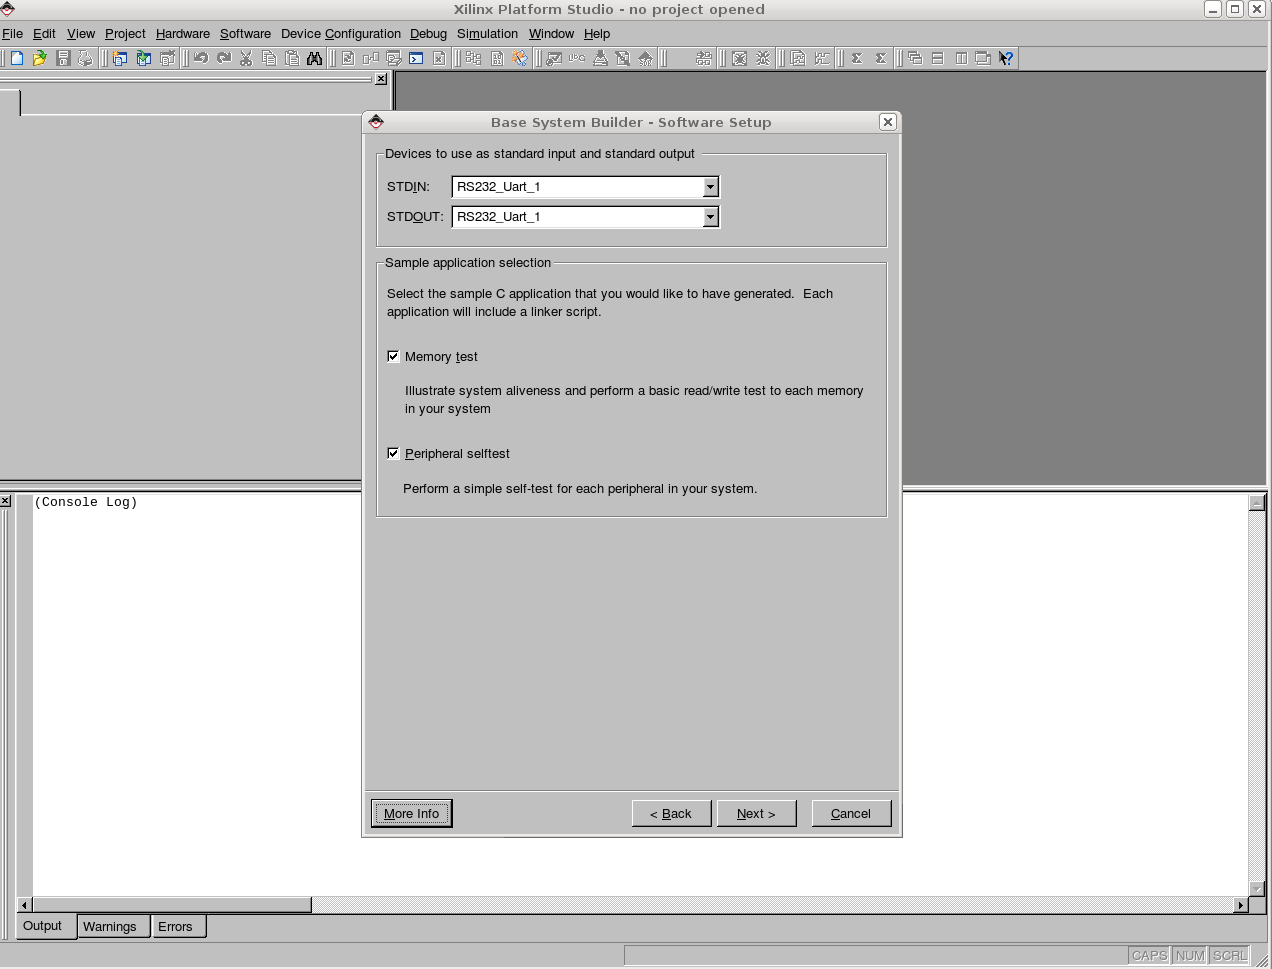
\includegraphics[scale=.25]{./figuras/EDK11.png}
  % capas.png: 607x522 pixel, 72dpi, 21.41x18.41 cm, bb=0 0 607 522
  \caption{Selección de división del programa en memoria}
  \label{Selección de división del programa en memoria}
  \end{figure}
  
  
\item Generación del \emph{hardware}, \emph{figura}\ref{Generación de hardware}.
  \begin{figure}[h!] 
  \centering
  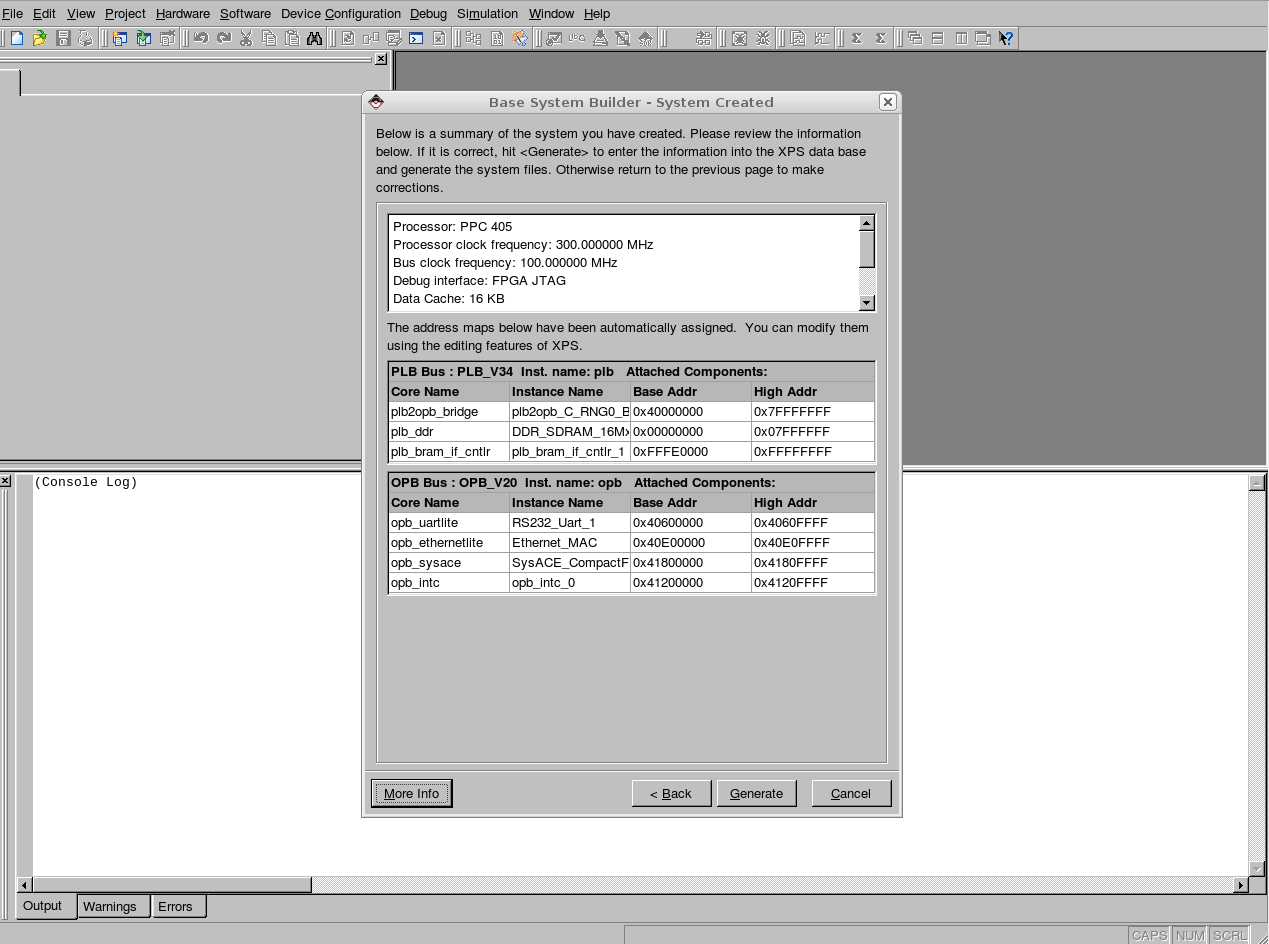
\includegraphics[scale=.25]{./figuras/EDK13.png}
  % capas.png: 607x522 pixel, 72dpi, 21.41x18.41 cm, bb=0 0 607 522
  \caption{Generación de \emph{hardware} }
  \label{Generación de hardware}
  \end{figure}
  
  
\item El siguiente paso es activar el doble buffer (también conocido como
``ping-pong'' buffers) para el núcleo opb\_ethernetlite (doble clic sobre
``Ethernet\_MAC'' de la \emph{``System Assembly View''}),
\emph{figura}\ref{Configuración del OPB EthernetLite}.
  \begin{figure}[h!] 
  \centering
  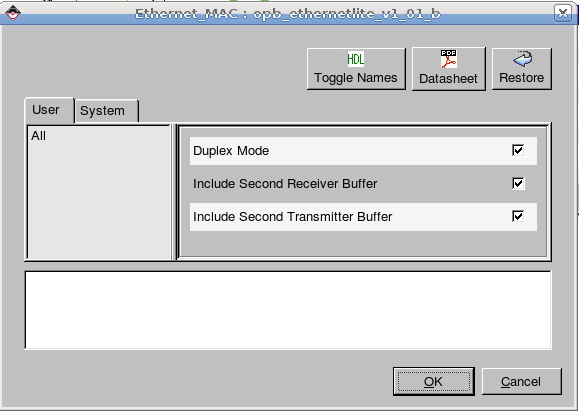
\includegraphics[scale=.25]{./figuras/pingpong.png}
  % capas.png: 607x522 pixel, 72dpi, 21.41x18.41 cm, bb=0 0 607 522
  \caption{Configuración del OPB\_EthernetLite}
  \label{Configuración del OPB EthernetLite}
  \end{figure}
  
  
\item Generación del proyecto( Opción de menú: \emph{``Device Configuration:
Update Bistream''}).
\item Habilite el \emph{bootloop} en la BRAM, dando click derecho en pestaña de
aplicaciones y seleccionando \emph{``Mark to initialize BRAM''},
\emph{figura}\ref{Confuración del bootloop}.
  \begin{figure}[h!] 
  \centering
  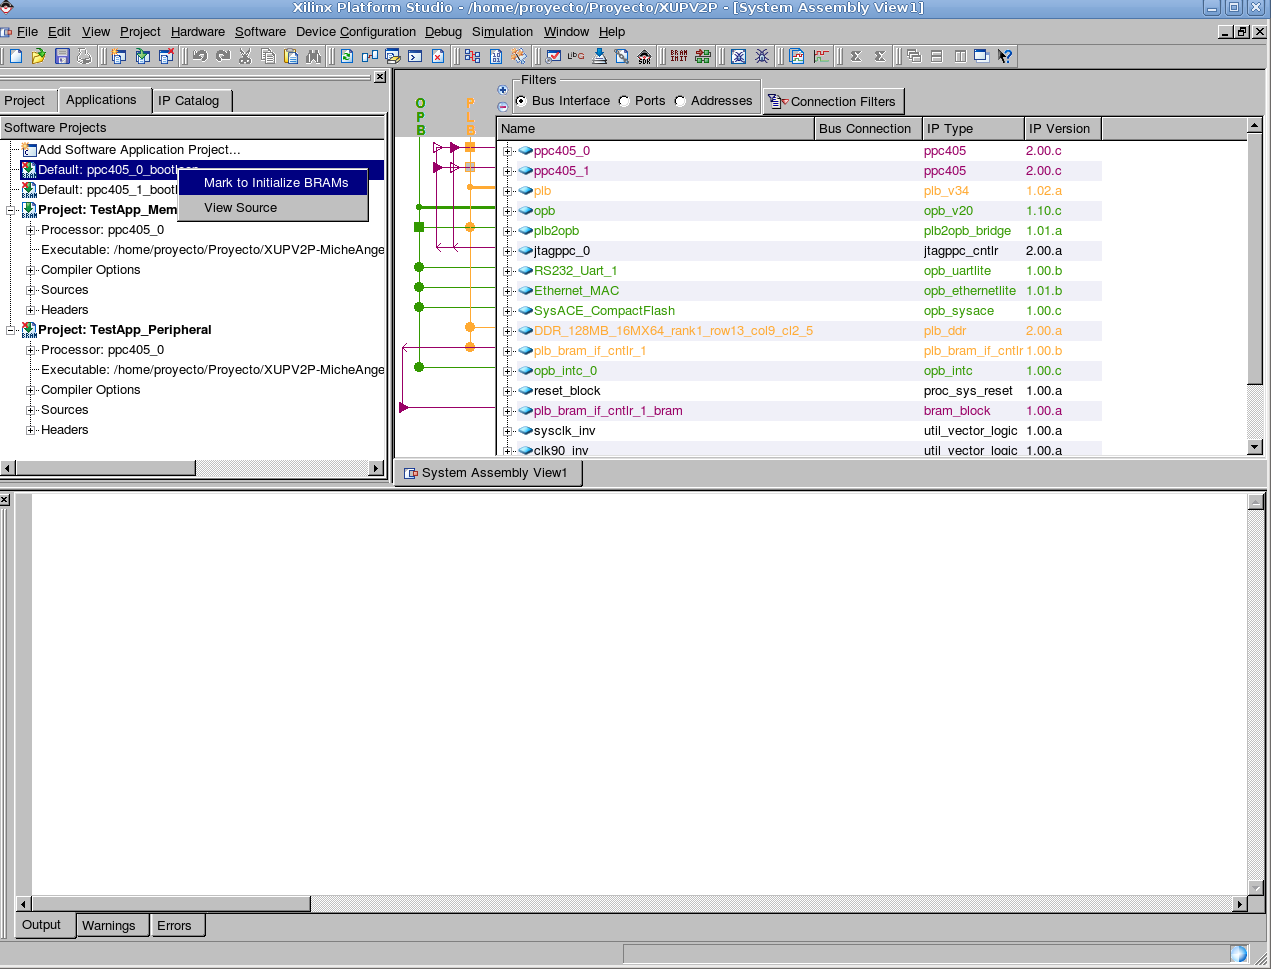
\includegraphics[scale=.25]{./figuras/bootloop.png}
  % capas.png: 607x522 pixel, 72dpi, 21.41x18.41 cm, bb=0 0 607 522
  \caption{Confuración del bootloop}
  \label{Confuración del bootloop}
  \end{figure}

\item Generar el árbol de dispositivos de Linux. Cuando haya terminado de
ejecutar el software de pruebas básicas, es hora de volver a configurar el
software en el proyecto de XPS para generar un árbol de dispositivos, necesario
para compilar un kernel de Linux a la medida. 

\item   Menú ``Software: Software Platform Settings...'' a
continuación, seleccione ``device-tree``, como el sistema operativo,
\emph{figura}\ref{devicetree}.
  \begin{figure}[h!] 
  \centering
  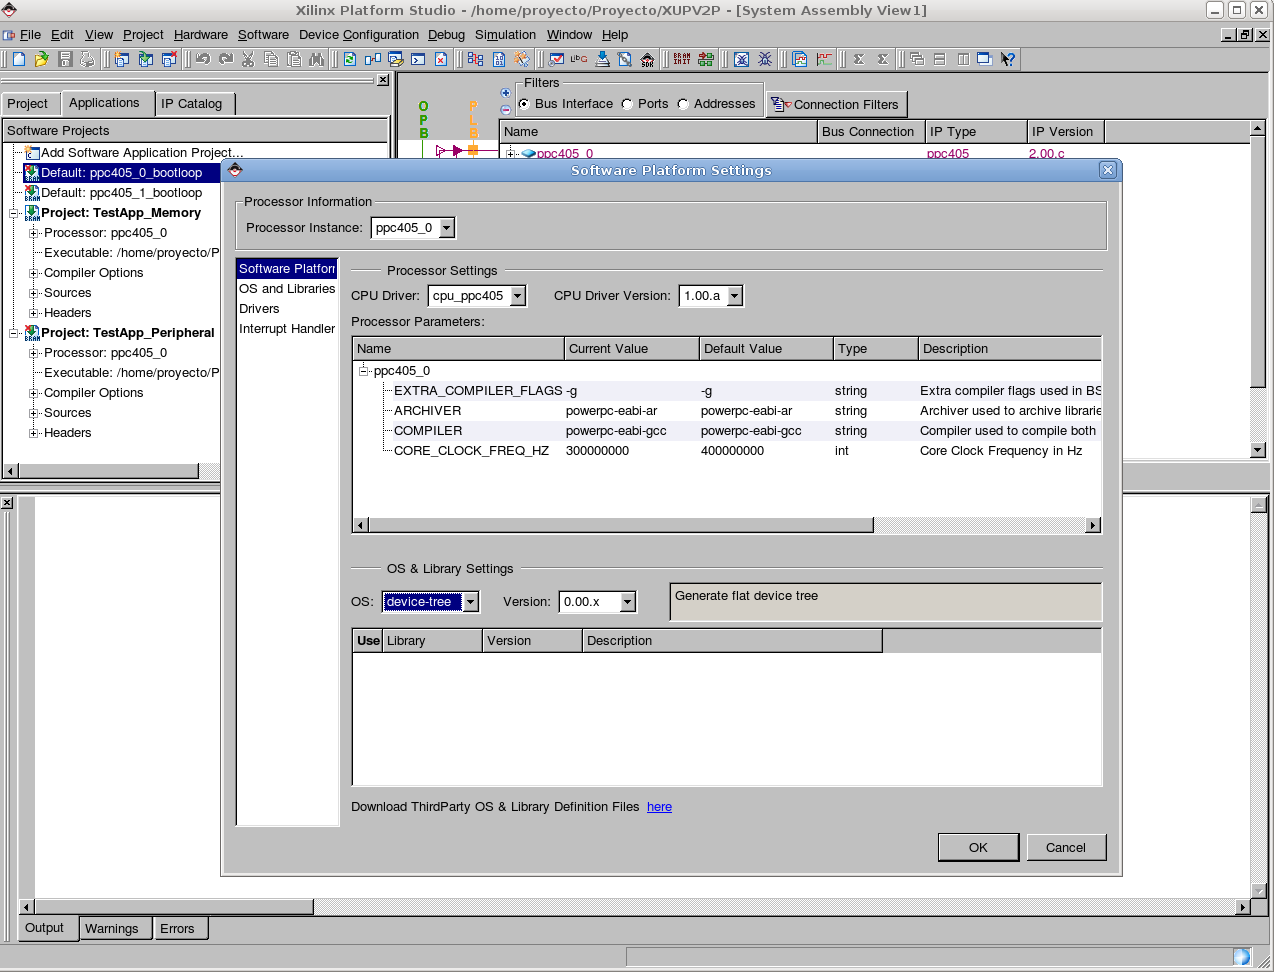
\includegraphics[scale=.25]{./figuras/devicetree.png}
  % capas.png: 607x522 pixel, 72dpi, 21.41x18.41 cm, bb=0 0 607 522
  \caption{Selección Device Tree}
  \label{devicetree}
  \end{figure}
  
  
\item Ajuste \emph{''console device''} a su UART. Actualizar \emph{``bootargs''}
para incluir \emph{console = ttyUL0, 115200}, \emph{figura}\ref{uart}.
  \begin{figure}[h!] 
  \centering
  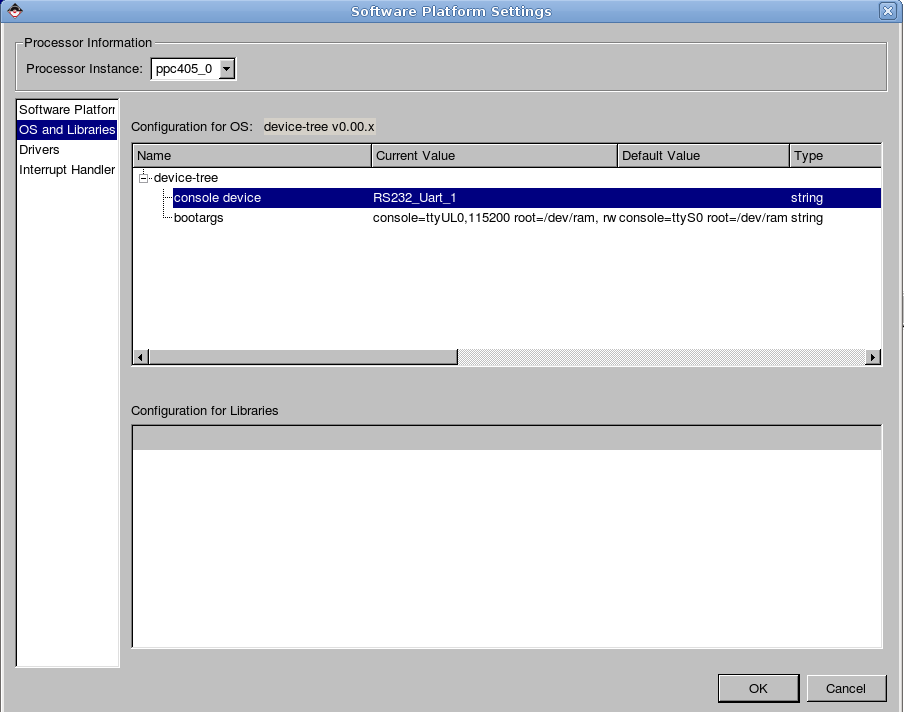
\includegraphics[scale=.25]{./figuras/uart.png}
  % capas.png: 607x522 pixel, 72dpi, 21.41x18.41 cm, bb=0 0 607 522
  \caption{BootArgs Kernel Command Line estática}
  \label{uart}
  \end{figure}
  
  
\item Generar el árbol de dispositivos, haga clic en el menú: \emph{``Software:
Generate Libraries and BSPs''}. El siguiente archivo se creará dentro de su
directorio del proyecto EDK: ./ppc405\_0/libsrc/device-tree/xilinx.dts. Este
archivo (xilinx.dts) se utilizará para ayudar a construir el kernel de Linux.

\end{enumerate}

El diseño final se puede apreciar en la figura\cite{system}, generada por el EDK

  \begin{figure}[h!] 
  \centering
  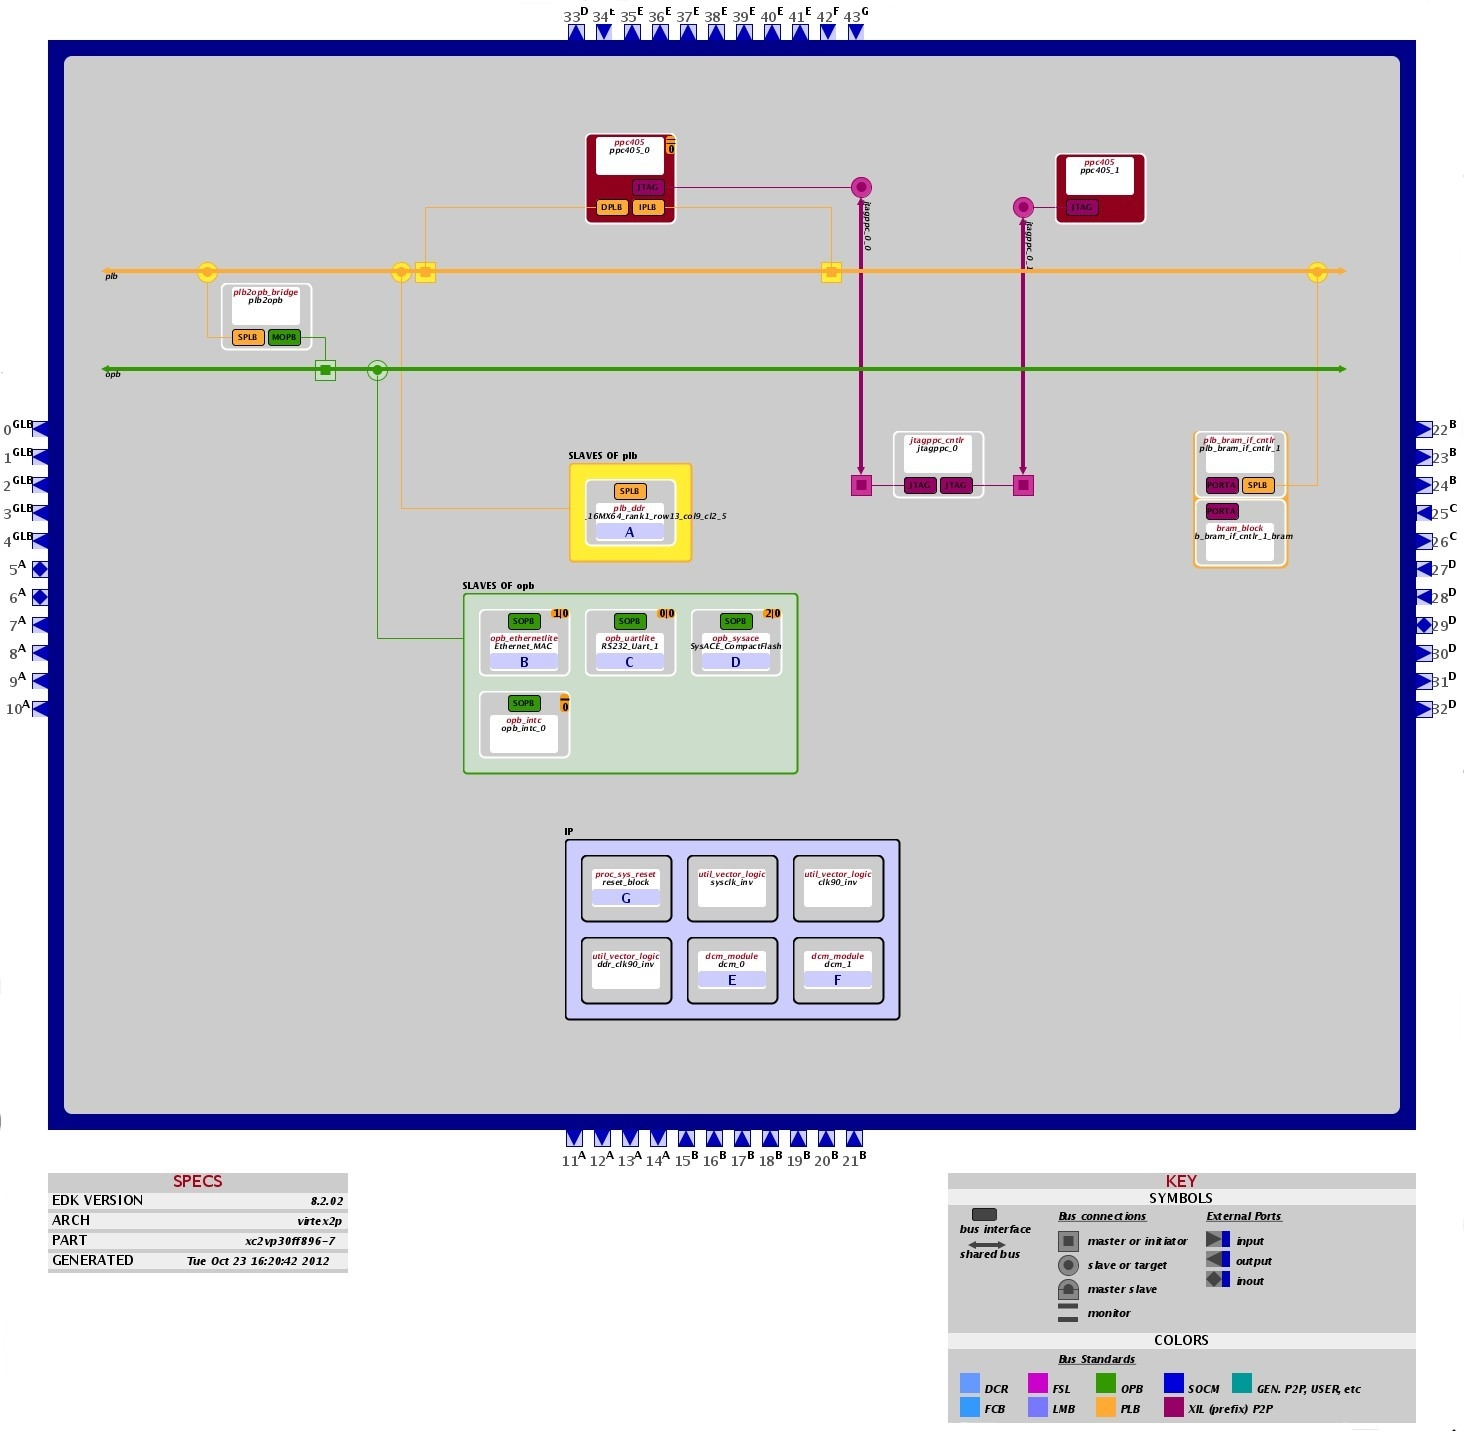
\includegraphics[scale=.40]{./figuras/system.jpg}
  % capas.png: 607x522 pixel, 72dpi, 21.41x18.41 cm, bb=0 0 607 522
  \caption{Diagrama de bloques del \emph{hardware} creado}
  \label{system}
  \end{figure}

\clearpage \newpage

\section{\emph{Device Tree File}}

El archivo xilinx.dts contine una descripción detallada del \emph{hardware}, un
mapa de memoria que permite acceder por DMA, el archivo ``xilinx.dts''
configurado se muestra en el \emph{Apéndice B}.

